A perturbációszámítás a Green-függvény egyik legjelentősebb alkalmazása. Ebben a részben a Green-függvény perturációs sorának a konvergencia tulajdonságait vizsgáljuk. A konvergencia tartományát és sebességét befolyásolja a perturbáló operátor triviális módosítása, konkrétan a vizsgált példában az $\frac{FL}{2}\op{I}$ operátort a perturbáló tagból levonjuk és a perturálatlan operátorhoz hozzáadjuk. Ezzel a teljes Hamilton operátor nem változik, de a perturbációs sor konvergenciája igen.

A perturbációszámításhoz a Hamilton operátort két részre bontjuk,
\begin{equation}
	\op{H} = \op{H}_0 + \op{V}.
\end{equation}
A $\op{H}_0$ operátorhoz tartozó rezolvens operátor $\op{G}_0\left(E\right)$. Mind $\op{H}$ és mind $\op{H}_0$ kifejezhetőek a rezolvenseikkel, ha ezeket behelyettesítjük a fenti egyenletbe, implicit egyenletet kapunk $\op{G}\left(E\right)$-re nézve,
\begin{equation}
	-\op{G}^{-1}\left(E\right) - E = -\op{G}_0^{-1}\left(E\right) - E + \op{V}.
\end{equation}
Ezt kisebb átalakítások után fel lehet használni perturbációszámításra. Az egyenletet balról $\op{G}_0\left(E\right)$-vel, jobbról $\op{G}\left(E\right)$-vel szorozzuk, így
\begin{equation}
	\op{G}\left(E\right) = \op{G}_0\left(E\right) + \op{G}_0\left(E\right)\op{V}\op{G}\left(E\right)
	\label{green:pertmaster}
\end{equation}
eredményhez jutunk. Megfelelően definiálva $\op{G}_n\left(E\right)$ operátorokat,
\begin{equation}
	\op{G}_n\left(E\right) = \op{G}_0\left(E\right)\sum_{k=0}^n\left(\op{V}\op{G}_0\left(E\right)\right)^k,
\end{equation}
a $\op{G}_n$-ekre \aeqref{green:pertmaster} egyenlethez hasonló rekurziós összefüggés áll fent,
\begin{equation}
	\op{G}_{n+1}\left(E\right) = \op{G}_0\left(E\right) + \op{G}_0\left(E\right)\op{V}\op{G}_n\left(E\right).
	\label{perturbation:rekurzió}
\end{equation}
Ha $\norm{\op{V}\op{G}_0\left(E\right)} < 1$ akkor a $\op{G}_n$ sorozat konvergál. Operátor normának a Hilbert-tér normája által indukált normát vesszük, így az operátorok konvergenciája kompatibilis a Hilbert-tér beli konvergenciával.
\begin{equation}
	\norm{\op{A}}=\sup \Set{\left\lvert \op{A}\Ket{\phi} \right\rvert \texttt{, ahol} \Braket{\phi|\phi}=1}.
\end{equation}
A sor határértéke \aeqref{perturbation:rekurzió} miatt kielégíti \aeqref{green:pertmaster} egyenletet. Így konvergencia esetén
\begin{equation}
	\op{G}\left(E\right) = \op{G}_0\left(E\right)\sum_{n=0}^\infty\left(\op{V}\op{G}_0\left(E\right)\right)^n.
\end{equation}
Ez azt jelenti, hogy ha egy operátornak van projektor felbontása, akkor a normája a legnagyobb sajátérték abszolút értéke lesz, vagy általános esetben a sajátértékek szuprémuma. Ez hasznos jelen esetben is, mivel így meg tudjuk határozni az $\op{V}=a\op{x}+b$ operátor normáját. Ennek az operátornak a sajátfüggvényei a $\delta(x-x_0)$ függvények, így a sajátértékek maximuma a $[0,L]$ tartományban
\begin{equation}
	\norm{\op{V}}=\max(\rvert b \lvert, \lvert aL+b\rvert).
\end{equation}
\Aeqref{green:greensum} egyenlet alapján $\op{G}(E)$ normája is meghatározható, az összeg nevezői közül kiválasztva a legkisebb abszolút értékűt,
\begin{equation}
	\norm{\op{G}(E)}=\frac{1}{E-E_k},
\end{equation}
ahol $E$-hez a komplex síkon a legközelebbi sajátérték $E_k$. Ezek segítségével felső korlátot lehet adni a $\norm{\op{G}_1\op{V}}$-re.

A Hamilton-operátort eredetileg
\begin{equation}
	\begin{aligned}
		\op{H}=&\frac{\op{p}^2}{2m}+F\op{x}=\op{H}_0+\op{V}_1\\
		\op{H}_0=&\frac{\op{p}^2}{2m}\\
		\op{V}_1=&F\op{x}
	\end{aligned}
\end{equation}
részekre bontottuk. $\op{G}_0$ a $\op{H}_0$ operátor Green-függvénye. Ebben ha az esetben a $\op{G}_0$ pólusaitól legalább $FL$ távolságban, azaz $\rvert E-E_k\lvert>FL$, a komplex energia síkban a sor garantáltan konvergál, mert
\begin{equation}
	\norm{\op{G}_0(E)V_1}<\norm{\op{G}_0}\norm{(E)V_1}=\frac{FL}{\rvert E-E_k\lvert}<1.
\end{equation}
Vizsgálunk egy módosított felontást is,
\begin{equation}
	\begin{aligned}
		\op{H}=&\frac{\op{p}^2}{2m}+F\op{x}=\op{H}_0+\frac{FL}{2}+\op{V}_2\\
		\op{H}_0=&\frac{\op{p}^2}{2m}\\
		\op{V}_2=&F\op{x}-\frac{FL}{2}.
	\end{aligned}
\end{equation}
A perturbációszámítás során így a perturbálatlan operátor szerepét a $\op{H}_0+\frac{FL}{2}$ operátor tölti be. Ennek a Green-függvénye
\begin{equation}
	\frac{1}{E-\left(\op{H}_0+\frac{FL}{2}\right)}=\op{G}_0(E-\frac{FL}{2}),
\end{equation}
könnyen kifejezhető az eredeti eset Green-függvényével.

A $\frac{\op{p}^2}{2m}$ Green-függvénye a $[0,L]$ tartományban \aref{egzakt}. fejezethez hasonlóan meghatározható,
\begin{equation}
	G_0\left(x,y;E\right) = -\frac{\hbar}{\sqrt{2m}}\frac{1}{\sin\left(kL\right)}\times
	\begin{cases}
		\sin\left(k\left(y-L\right)\right)\sin\left(kx\right) & x\leq y\\
		\sin\left(k\left(x-L\right)\right)\sin\left(ky\right) & x\geq y\\
	\end{cases},
\end{equation}
\begin{equation}
	k = \frac{\sqrt{2mE}}{\hbar}.
\end{equation}

\begin{figure}[H]
	\centering
	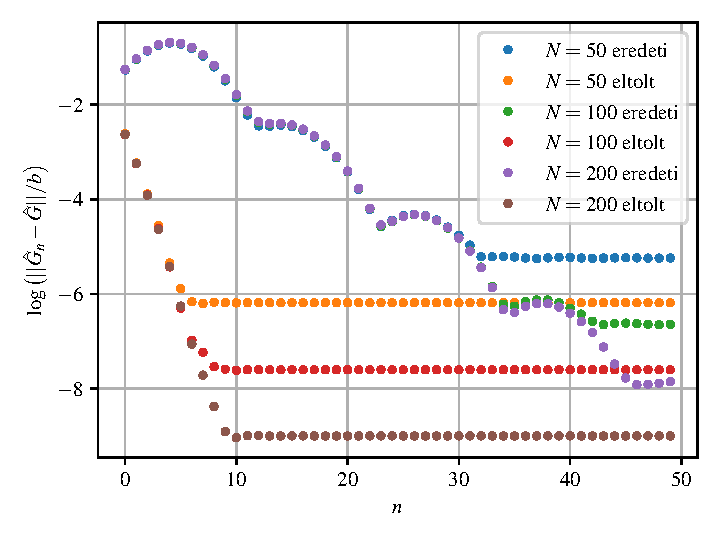
\includegraphics[scale=1]{./figs/convergencerate.pdf}
	\caption[A Green-függvény perturbációs sorának konvergencia sebessége]{ye, awesome}
\end{figure}
\begin{figure}[H]
	\centering
	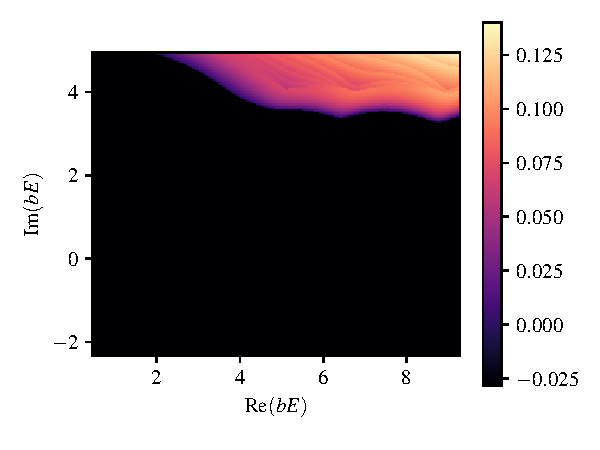
\includegraphics[scale=1]{./figs/convergenceOriginal.pdf}
	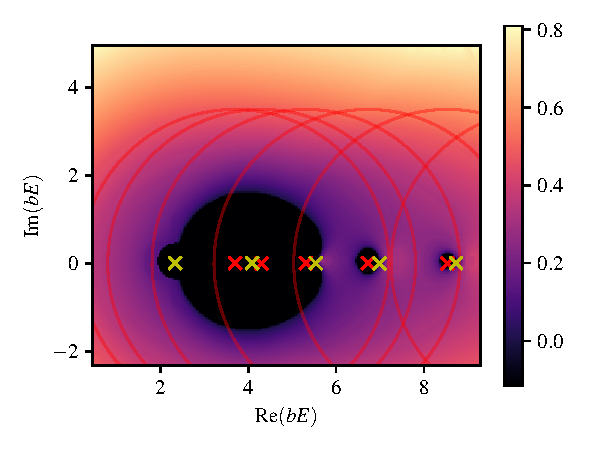
\includegraphics[scale=1]{./figs/convergenceImproved.pdf}
	\caption[A Green-függvény perturbációs sorának konvergenciatartománya]{Ez az ábra a két perturbációs sor konvergenciáját hasonlítja össze a komplex energia síkon. A felső ábra a $V=Fx$ perturbáló potenciálnak, míg az alsó a $V = Fx-FL/2$ perturbáció szerinti sornak felel meg. A fekete tartományok divergenciát jelölnek, míg a többi szín a sorfejtés tagjainak csökkenési sebességét jellemzik, a norma harmadolásához szükséges lépések számát megadva. A piros körökön kívüli tartomány a ?? formula által garantált konvergencia tartományát jelöli. A piros x-ek a $\hat{G}_0$ pólusait, a sárga x-ek pedig az egzakt $\hat{G}$ operátor pólusait jelölik.}
\end{figure}